% ---------
%  Compile with "pdflatex hw0".
% --------
%!TEX TS-program = pdflatex
%!TEX encoding = UTF-8 Unicode

\documentclass[11pt]{article}
\usepackage{jeffe,handout,graphicx}
\usepackage[utf8]{inputenc}		% Allow some non-ASCII Unicode in source
\usepackage{amsmath}
\usepackage[makeroom]{cancel}
\usepackage{tikz}
\usetikzlibrary{arrows,automata}

%  Redefine suits
\usepackage{pifont}
\def\Spade{\text{\ding{171}}}
\def\Heart{\text{\textcolor{Red}{\ding{170}}}}
\def\Diamond{\text{\textcolor{Red}{\ding{169}}}}
\def\Club{\text{\ding{168}}}

\def\Cdot{\mathbin{\text{\normalfont \textbullet}}}
\def\Sym#1{\textbf{\texttt{\color{BrickRed}#1}}}



% =====================================================
%   Define common stuff for solution headers
% =====================================================
\Class{CS/ECE 374}
\Semester{Fall 2018}
\Authors{2}
\AuthorOne{Will Koster}{jameswk2@illinois.edu}
%\Section{}

% =====================================================
\begin{document}

% ---------------------------------------------------------


\HomeworkHeader{2}{1}	% homework number, problem number

\begin{quote}
    \begin{enumerate}
        \item Draw an NFA that accepts the language $\{w \mid$ there is exactly one  block of 1s of odd length\}.  (A ``block of 1s'' is a maximal substring of 1s.)
        \item
            \begin{enumerate}
                \item Draw an NFA for the regular expression $(010)^* + (01)^* + 0^*$.
                \item Now using the powerset construction (also called the subset
                    construcion), design a DFA for the same language.  Label the states
                    of your DFA with names that are sets of states of your NFA. You
                    should use the incremental construction so that you only generate
                    the states that are reachable form the start state.
            \end{enumerate}
    \end{enumerate}
\end{quote}
\hrule



\begin{solution}
    \begin{enumerate}
        \item
    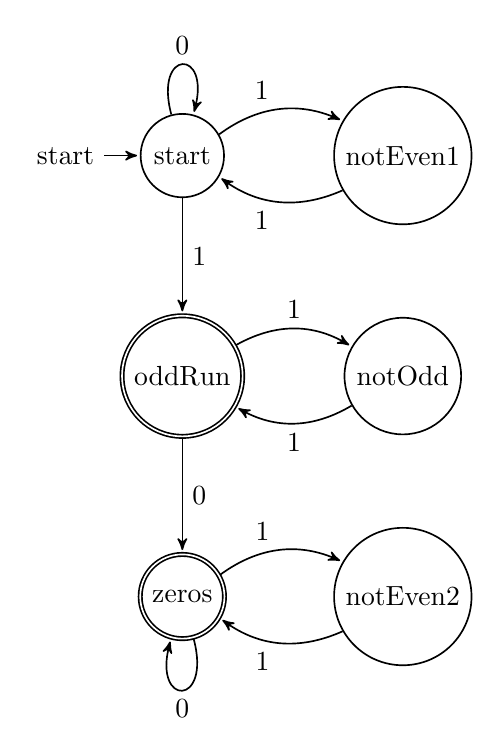
\begin{tikzpicture}[->,>=stealth',shorten >=1pt,auto,node distance=2.8cm,
                    semithick]
   \node[state,initial] (start)   {start};
   \node[state] (oddOnes1) [right of=start] {notEven1};
   \node[state,accepting] (oddRun) [below of=start] {oddRun};
   \node[state] (midOddRun) [right of=oddRun] {notOdd};
   \node[state,accepting] (zerosAfter) [below of=oddRun] {zeros};
   \node[state](oddOnes2) [right of=zerosAfter] {notEven2};
    \path[->]
    (start) edge [loop above] node {0} ()
    edge [bend left] node {1} (oddOnes1)
    edge  node {1} (oddRun)
    (oddOnes1) edge [bend left]  node  {1} (start)
    (oddRun) edge [bend left] node  {1} (midOddRun)
    edge node {0} (zerosAfter)
    (midOddRun) edge [bend left] node {1} (oddRun)
    (zerosAfter) edge [loop below] node {0} ()
    edge [bend left] node {1} (oddOnes2)
    (oddOnes2) edge [bend left] node {1} (zerosAfter);

\end{tikzpicture}
\item 
    \begin{enumerate}
        \item
            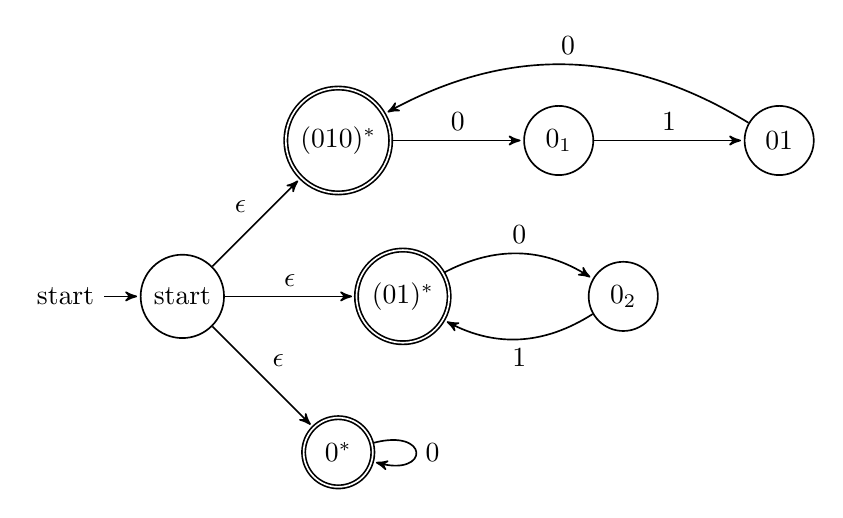
\begin{tikzpicture}[->,>=stealth',shorten >=1pt,auto,node distance=2.8cm,
                    semithick]
                \node[state,initial] (start)   {start};
                \node[state,accepting] (e1) [above right of=start] {$(010)^*$};
                \node[state] (zero1) [right of=e1] {$0_1$};
                \node[state] (zeroone1) [right of=zero1] {01};

                \node[state,accepting] (e2) [right of=start] {$(01)^*$};
                \node[state] (zero2) [right of=e2] {$0_2$};

                \node[state,accepting] (e3) [below right of=start] {$0^*$};

    \path[->]
    (start) edge node {$\epsilon$} (e1)
    edge node {$\epsilon$} (e2)
    edge node {$\epsilon$} (e3)

    (e1) edge node {0} (zero1)
    (zero1) edge node {1} (zeroone1)
    (zeroone1) edge [bend right] node [swap] {0} (e1)

    (e2) edge [bend left] node {0} (zero2)
    (zero2) edge [bend left] node {1} (e2)

    (e3) edge [loop right] node {0} ();
            \end{tikzpicture}
        \item
            \iffalse
            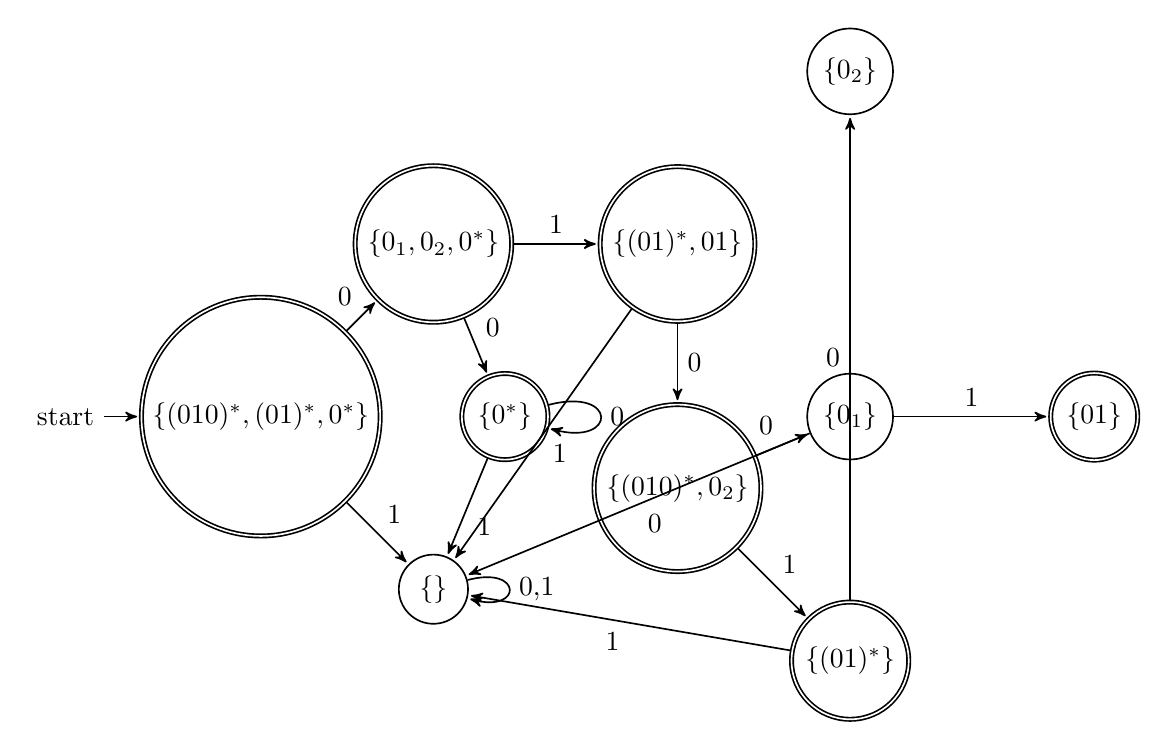
\begin{tikzpicture}[->,>=stealth',shorten >=1pt,auto,node distance=3.1cm,
                    semithick]
                \node[state,initial, accepting] (start)   {$\{(010)^*,(01)^*,0^*\}$};
                \node[state, accepting] [above right of=start] (z1z2zs)   {$\{0_1,0_2,0^*\}$};
                \node[state] [below right of=start] (empty) {$\{\}$};
                \node[state, accepting] [right of=start] (zs)   {$\{0^*\}$};
                \node[state, accepting] [right of=z1z2zs] (zerooneszeroone)   {$\{(01)^*,01\}$};
                \node[state, accepting] [below of=zerooneszeroone] (zerooneszeroone2)   {$\{(010)^*,0_2\}$};
                \node[state] [below right of=zerooneszeroone] (zeroone) {$\{0_1\}$};
                \node[state] [above right of=zerooneszeroone] (zerotwo) {$\{0_2\}$};
                \node[state,accepting] [below right of=zerooneszeroone2] (zos) {$\{(01)^*\}$};
                \node[state,accepting] [right of=zeroone] (zo) {$\{01\}$};
                \path[->]
                (start) edge node {0} (z1z2zs)
                edge node {1} (empty)
                (z1z2zs) edge node {1} (zerooneszeroone)
                edge node {0} (zs)
                (empty) edge [loop right] node {0,1} ()
                (zs) edge [loop right] node {0} ()
                edge node {1} (empty)
                (zerooneszeroone) edge node {1} (empty)
                edge node {0} (zerooneszeroone2)
                (zerooneszeroone2) edge node {0} (zeroone)
                edge node {1} (zos)
                (zos) edge node {0} (zerotwo)
                edge node {1} (empty)
                (zeroone) edge node {0} (empty)
                edge node {1} (zo);
                \end{tikzpicture}
                \fi
                Let $M = (Q, \Sigma, \delta, s, A)$ be our new DFA for this language.\\ 
                Let $N = (Q', \Sigma, \delta',s',A')$ be the NFA we built above. \\
                \[
                    \delta(qs, x) = \bigcup_{q \in qs}\bigcup_{r \in \epsilon reach(q)} \epsilon reach(\delta'(r, x))
                \]
                Note that $\delta^*: Q \times \Sigma^* \rightarrow \mathbb{P}(Q')$ is the standard string extension of our $\delta$ function.
                \[
                    Q = \{\delta^*(s, w) : w \in \Sigma^*\}
                \]
                \[
                    s = \epsilon reach(s')
                \]
                \[
                    A = \{ a : a \subseteq Q, a \cap A' \neq \emptyset\}
                \]
    \end{enumerate}
\end{enumerate}
\end{solution}

\HomeworkHeader{2}{2}	% homework number, problem number

\begin{quote}
    In Lab 3 we considered the language
  $\emph{delete}\Sym1(L) = \{xy \mid x\Sym1y \in L\}$.  Intuitively,
  $\emph{delete}\Sym1(L)$ is the set of all strings that can be
  obtained from strings in $L$ by deleting exactly one \Sym1.  For
  example, if $L = \set{\Sym{101101}, \Sym{00}, \e}$, then
  $\emph{delete}\Sym1(L) = \set{\Sym{01101}, \Sym{10101},
    \Sym{10110}}$.  We argued that if $L$ is regular then
  $\emph{delete}\Sym1(L)$ is also regular and the proof strategy was
  as follows: given a DFA $M$ such that $L=L(M)$, construct an NFA
  $N$ such that $L(N) = \emph{delete}\Sym1(L)$. Here we consider a
  different proof technique.  Let $r$ be a regular expression. We
  will develop an algorithm that given $r$ constructs a regular expression
  $r'$ such that $L(r') = \emph{delete}\Sym1(L(r))$. Assume
  $\Sigma = \{\Sym0,\Sym1\}$.
    \begin{enumerate}
    \item For each of the base cases of regular expressions
      $\emptyset, \epsilon$ and $\{a\}, a \in \Sigma$ describe
      a regular expression for $\emph{delete}\Sym1(L(r))$.
    \item Suppose $r_1$ and $r_2$ are regular expressions, and
      $r'_1$ and $r'_2$ are regular expressions for the languages
      $\emph{delete}\Sym1(L(r_1))$ and $\emph{delete}\Sym1(L(r_2))$
      respectively. Describe a regular expression for the language
      $\emph{delete}\Sym1(L(r_1+r_2))$ using $r_1,r_2,r'_1,r'_2$.


      Briefly justify the correctness of your construction.
      The argument should take the form of proving $L_1 = L_2$ by
      showing that $L_1 \subseteq L_2$ and $L_2 \subseteq L_1$.

    \item Same as the previous part but now consider $L(r_1r_2)$. This
      is a bit more tricky than the previous part.
    \item Same as the previous part but now consider $L((r_1)^*)$.
    \item Apply your construction to the regular expression
      $r = 0^* + (01)^*+ 011^*0$ to obtain a regular expression for
      the language $\emph{delete}\Sym1(L(r))$.
  \end{enumerate}
\end{quote}
\hrule



\begin{solution}
    \begin{enumerate}
        \item The set for the regular expression $\emptyset$ is empty, so the regular expression for $\emph{delete}\Sym{1}(\emptyset)$ is trivially also $\emptyset$. The set for $\epsilon$ only has one string in it, and there are no $\Sym1$s in it to remove, so $\emph{delete}\Sym{1}(\epsilon)$ is also $\emptyset$. There are two 1-letter regular expressions in this language, $\Sym1$ and $\Sym0$. $\emph{delete}\Sym1(\Sym1) = \epsilon$ and $\emph{delete}\Sym1(\Sym0) = \emptyset$.

        \item The regular expression is $r_1' + r_2'$. If we take some string $w$ from $\emph{delete}\Sym1(L(r_1+r_2))$, it is by definition some string from either $L(r_1)$ or $L(r_2)$ with a 1 removed. Since our regular expression matches strings from either $L(r_1)$ or $L(r_2)$ that have had a $1$ removed, w is in $L(r_1' + r_2')$. Therefore, if any string that is in $\emph{delete}\Sym1(L(r_1+r_2))$ is in $L(r_1' + r_2')$, then $\emph{delete}\Sym1(L(r_1+r_2)) \subseteq L(r_1' + r_2')$. Similarly, if we take some string $p$ from $L(r_1' + r_2')$, by the definition of $r_1'$ and $r_2'$, it is either a string from $L(r_1)$ or $L(r_2)$ with a $1$ removed. This means that string will be in $\emph{delete}\Sym1(L(r_1+r_2))$, so $L(r_1' + r_2') \subseteq \emph{delete}\Sym1(L(r_1+r_2))$. Therefore, the languages are the same.

        \item The regular expression is $r_1'r_2 + r_1r_2'$. Let $P = L(r_1'r_2 + r_1r_2')$ and $D = \emph{delete}\Sym1(L(r_1r_2))$. If you take some string from $P$, then it will either be something matching $r_1$, but with a $1$ removed, followed by something matching $r_2$, or something matching $r_1$ followed by something matching $r_2$ but with a $1$ deleted. If you put the $1$ back, then you have something matching $r_1$ followed by something matching $r_2$, which means that the original string is in $D$. If you take a some string matching $r_1r_2$ and then delete a $1$, that $1$ could have come from the $r_1$ part or the $r_2$ part, which means that string also would be in $P$. Therefore, $P = D$.
            
        \item The regular expression is $(r_1)^*r_1'(r_1)^*$. Let $P = L((r_1)^*r_1'(r_1)^*)$ and $D = \emph{delete}\Sym1(L((r_1)^*))$. Let $w$ be some string from $P$. If you find the part of the string that matches $r_1'$ and replace the $1$ to make it match $r_1$, giving you a string $w_1$, then $w_1$ is in $L((r_1)^*)$. That means that $w$ is in $D$. If you take some new string $r$ from $D$, you know that it's the concatenation of some number of strings that match $(r_1)^*$ with a single $1$ removed. That means that one of the repetitions of $r_1$ turns into an $r_1'$ and the rest stay how they were, which is the definition of $P$. Therefore, $r \in P$ and $P = D$.
            
        \item $(01)^*0(01)^* + 01*0$
    \end{enumerate}
\end{solution}

\HomeworkHeader{2}{3}	% homework number, problem number

\begin{quote}
    \begin{enumerate}
  \item Suppose $M_1=(Q_1,\Sigma, \delta_1, s_1, A_1)$ is a DFA and
    $N_2=(Q_2,\Sigma, \delta_2, s_2, A_2)$ is an NFA. Formally
    describe a DFA that accepts the language
    $L(M_1) \setminus L(N_2)$. To be more specific, letting
    $M = (Q,\Sigma,\delta,s,A)$ be the DFA, describe the components
    $Q,\delta,s,A$ in terms of the components of $M_1$ and $N_2$.
    This combines subset construction and product construction to give
    you practice with formalism. Be aware of the distinction between
    the transition function of a DFA and that of a NFA. You can use
    $\delta_1^*$ and $\delta_2^*$ in your construction. You do not
    need to prove the correctness of your construction.
  \item For a language $L$ let
    $\text{SUFFIX}(L) = \{ y \mid \exists x \in \Sigma^*, xy \in L\}$ be
    the set of suffixes of strings in $L$.  Let
    $\text{PSUFFIX}(L) = \{ y \mid \exists x \in \Sigma^*, |x| \ge 1, xy
    \in L\}$ be the set of proper suffixes of strings in $L$.  Prove
    that if $L$ is regular then $\text{PSUFFIX}(L)$ is regular via the
    following technique.  Let $M=(Q,\Sigma,\delta,s,A)$ be a DFA
    accepting $L$. Describe a NFA $N$ in terms of $M$ that accepts
    $\text{PSUFFIX}(L)$. Explain the construction of your NFA.
  \end{enumerate}
\end{quote}
\hrule



\begin{solution}
    \begin{enumerate}
        \item First, let's build $M_2$, the conversion of $N_2$ to a DFA.
            \[
                M_2 = (Q_2', \Sigma, \delta_2', s_2', A_2')
            \]
            \[
                Q_2' = \mathbb{P}(Q_2)
            \]
            \[
                \delta_2'(qs, a) = \bigcup_{q \in qs}\left(\bigcup_{r \in \epsilon reach(q)} \epsilon reach(\delta'(r, x))\right)
            \]
            \[
                s_2' = \epsilon reach(s_2)
            \]
            \[
                A_2' = \{q : q \in Q_2', q \cap A_2 \neq \emptyset \}
            \]
            Now we're going to create a DFA $F$ that accepts $L(M_1) \setminus L(M_2)$.
            \[
                F = (Q_3, \Sigma, \delta_3, s_3, A_3)
            \]
            \[
                Q_3 = Q_1 \times Q_2'
            \]
            \[
                \delta_3((a,b),c) = (\delta_1(a, c), \delta_2'(b,c))
            \]
            \[
                s_3 = (s_1, s_2')
            \]
            \[
                A_3 = \{(a, b) \in Q_3 : a \in A_1, b \in \overline{A_2'}\}
            \]
        \item The intuition behind $N$ is that it will be just like $M$ except there will be a new start state $s'$ that has $\epsilon$ transitions to every state reachable from $s$. Also, let $\delta^*$ be the standard extension of $\delta$ to strings.
            \[
                N = (Q', \Sigma, \delta', s',A)
            \]
            \[
                Q' = Q \cup \{s'\}
            \]
            \[
                \delta'(s', \epsilon) = \{\delta^*(s, w) : w \in \Sigma^*\}
            \]
            \[
                \delta'(s', x) = \emptyset
            \]
            \[
                \delta'(q, a) = \{\delta(q, a)\}
            \]
    \end{enumerate}
\end{solution}
\end{document}
